% =====================================================================
%  ICDEC 2026  ---  Springer Lecture Notes in Networks and Systems (LNNS)
%  Class: llncs (Springer Proceedings LaTeX2e). Available in TeX Live and
%  on Overleaf, so this project compiles on upload with no extra files.
%  Length target: 10 pages (min 8, max 12) including figures and references.
% =====================================================================
\documentclass[runningheads]{llncs}

\usepackage{graphicx}
\usepackage{booktabs}
\usepackage{amsmath}
\usepackage{amssymb}
\usepackage[T1]{fontenc}
\usepackage{hyperref}
\renewcommand\UrlFont{\color{blue}\rmfamily}

\usepackage{placeins}   % \FloatBarrier

% Float control. With [t]-only placement LaTeX can defer a float past the end of
% the document and drop it ("Float(s) lost"). These settings let floats sit on a
% text page and keep them near the text that cites them.
\renewcommand{\topfraction}{0.90}
\renewcommand{\bottomfraction}{0.70}
\renewcommand{\textfraction}{0.10}
\renewcommand{\floatpagefraction}{0.75}
\setcounter{topnumber}{3}
\setcounter{bottomnumber}{2}
\setcounter{totalnumber}{5}

\graphicspath{{figures/}}

\begin{document}

\title{When Does a Second Variance Factor Pay? Pre-Registered Evidence
from Five Cryptocurrency Option Markets}

\titlerunning{When Does a Second Variance Factor Pay?}

% ---- REPLACE with your own author block -----------------------------
\author{First Author\inst{1}\orcidID{0000-0000-0000-0000} \and
Second Author\inst{1}}

\authorrunning{F. Author et al.}

\institute{Your Department, Your Institute, City, Country\\
\email{your.email@institute.edu}}
% ---------------------------------------------------------------------

\maketitle

\begin{abstract}
Two-factor stochastic volatility models are widely believed to price options
better than one-factor models, because they can represent a fast and a slow
source of variance at the same time. That belief is rarely tested in a way that
could have falsified it. We report a pre-registered comparison of
Black--Scholes, the Heston model and the Double-Heston model on 16,186 held-out option
quotes drawn from five cryptocurrency markets on the Deribit venue: Bitcoin,
Ether, Solana, XRP and Hyperliquid. Every evaluation date was selected from
volatility-index or spot data before any option data was downloaded, every
model was calibrated separately on each date, and accuracy was measured only on
quotes and expiries withheld from calibration. Significance required a
one-sided Wilcoxon signed-rank test \emph{and} a cluster-bootstrap lower bound
above zero, so that neither test alone could produce a result. The
Double-Heston model beat Black--Scholes on every asset, reducing median
implied-volatility error from 8.13 to 1.86 volatility points on Bitcoin shock
dates. Against the one-factor Heston model the picture differs sharply: Double
Heston won decisively on Bitcoin and Ether and failed to win on Solana, XRP and
Hyperliquid. The two markets where it won are the two that quote six to seven
expiries per day; the three where it did not quote about four. We argue that
the second variance factor pays only when the surface contains enough distinct
maturities to identify two mean-reversion speeds, and that reporting only
favourable markets conceals this boundary.

\keywords{Stochastic volatility \and Double Heston \and Option pricing \and
Cryptocurrency derivatives \and Model identifiability \and Pre-registration}
\end{abstract}

% =====================================================================
\section{Introduction}

Anyone pricing options must decide how much structure to buy. The
Black--Scholes formula assumes a single constant volatility and is wrong in a
way every practitioner can see: implied volatility varies with both strike and
maturity. The Heston model replaces that constant with one mean-reverting
variance process and captures much of the variation. A natural next step is to
add a second variance process on a different time scale, which is what the
Double-Heston model does. The motivation is intuitive. Short-dated options
respond to volatility that mean-reverts quickly, long-dated options to a slower
component, and one process cannot be fast and slow at once.

The argument is appealing, but the extra factor is not free. It doubles the
variance parameters from five to ten, and those parameters must be recovered
from a finite set of quoted prices. If the quoted surface does not contain
enough distinct maturities, two mean-reversion speeds cannot be told apart, and
the additional flexibility buys nothing while making calibration harder.
Whether the trade is worthwhile is therefore an empirical question, and it is a
question about the \emph{data} as much as about the model.

Most published comparisons answer it on one market, usually a major equity
index, and report a favourable result. Such a design cannot reveal where the
advantage stops. Our study is built to locate that boundary rather than to
demonstrate the advantage. We test the same three models on five
cryptocurrency markets that differ sharply in how many expiries they quote, and
we fix every choice that could bias the outcome before observing any option
price.

Our contributions are:

\begin{enumerate}
\item A pre-registered, five-market comparison of Black--Scholes, Heston and
Double Heston in which the evaluation dates were selected from volatility or
spot data before any option data was fetched, and the success criterion was
fixed in advance.
\item Evidence that the Double-Heston advantage over Black--Scholes is large
and universal across these markets, while its advantage over one-factor Heston
is \emph{conditional} and appears only where the surface quotes roughly six or
more expiries per day.
\item An identifiability explanation for that boundary, supported by the
negative results, including one market in which the one-factor model is
significantly better.
\item Full disclosure of a defect found in our own baseline implementation,
the frozen correction, and both sets of results.
\end{enumerate}

We do not claim that Double Heston is the best available model, that these
results transfer to equity or foreign-exchange markets, or that they imply a
trading strategy. We claim something narrower: the value of a second variance
factor depends on whether the market supplies enough maturities to estimate it.

% =====================================================================
\section{Related Work}

The Black--Scholes framework \cite{black1973} and Merton's analysis of rational
option pricing \cite{merton1973} establish classical option-valuation
foundations. Black's forward/futures option formulation \cite{black1976} is
relevant to the contract conventions considered here. Observed variation in
implied volatility across strikes and maturities motivates models beyond
constant volatility, as discussed by Gatheral \cite{gatheral2006}.

Heston \cite{heston1993} introduced a tractable stochastic-volatility model in
which variance follows a correlated square-root process. Bakshi, Cao and Chen
\cite{bakshi1997} evaluated extensions incorporating stochastic volatility,
stochastic interest rates and jumps on S\&P 500 options, finding that their
implications differ across pricing and hedging performance. Bates
\cite{bates2000} investigated post-crash concerns in the S\&P 500
futures-option market, while Duffie, Pan and Singleton \cite{duffie2000}
developed transform methods for affine jump-diffusion models. Particularly
relevant to the present comparison, Christoffersen, Heston and Jacobs
\cite{chj2009} showed how multiple stochastic-volatility factors can better
capture both the shape and term structure of equity-index option smiles. Their
work motivates testing whether a second variance factor provides a measurable
benefit beyond a one-factor model; it does not, by itself, establish that such
a benefit holds across cryptocurrency markets.

Efficient evaluation and stable calibration are essential for making this
comparison meaningful. Carr and Madan \cite{carr1999} developed an FFT-based
option-valuation method, and Fang and Oosterlee \cite{fang2008} introduced
Fourier-cosine expansions. Lord and Kahl \cite{lord2010} investigated the
treatment of complex logarithms in Heston-like characteristic functions, while
Cui, del Ba\~{n}o Rollin and Germano \cite{cui2017} studied efficient Heston
calibration. Feller's work on singular diffusion boundaries \cite{feller1951}
provides background for the treatment of the square-root variance boundary;
whether a Feller constraint is imposed is a separate modelling and calibration
choice.

Cryptocurrency options present an important empirical setting for this
question. Madan, Reyners and Schoutens \cite{madan2019} compared several
calibrated models, including Black--Scholes, variance-gamma-related models and
Heston, using Bitcoin option data. Hou and coauthors \cite{hou2020}
investigated cryptocurrency-option pricing with stochastic volatility and
correlated jumps, highlighting the role of jumps and co-jumps. Alexander and
Imeraj \cite{alexander2021} constructed Bitcoin implied-volatility indices from
Deribit option observations and examined the associated variance risk premia;
their subsequent study \cite{alexander2023} evaluated dynamic delta hedging
with smile-adjusted measures. These studies establish relevant cryptocurrency
option-pricing and volatility dynamics, but they do not directly answer the
specific question considered here: how the held-out benefit of a second Heston
variance factor changes across several cryptocurrency markets with different
maturity coverage.

Our evaluation therefore compares a term-structure Black baseline,
single-factor Heston and two-factor Heston using predefined calibration and
held-out partitions, including withholding entire expiries. Because multiple
dates may belong to the same market episode, paired comparisons are evaluated
at the cluster level. Wilcoxon's signed-rank procedure \cite{wilcoxon1945},
bootstrap inference \cite{efron1979} and clustered-resampling methodology
\cite{cameron2008} motivate the stated statistical checks. The frozen protocol
follows the broader rationale for preregistered research decisions
\cite{nosek2018}; Section~4 states the configuration, the freeze record and the
manifests that support the pre-data-freeze claim.

\section{Models and Numerical Method}

All models are priced in a forward-normalised, undiscounted convention. With
$F$ the forward price at the option's expiry, $K$ the strike,
$x=\log(F/K)$ the log-forward moneyness and $\tau$ the time to maturity in
years, we work with the normalised call value $c = C/F$. This removes the
discount factor and the level of the underlying from the comparison and matches
how the venue quotes its contracts.

\subsection{Black--Scholes with a Term Structure}

The constant-volatility model is given one volatility \emph{per expiry} rather
than one for the whole surface. This is a deliberately generous baseline: it
absorbs the entire maturity dimension of the smile and leaves only the strike
dimension unexplained. A quote in a calibrated expiry is priced with that
expiry's volatility; a quote in a withheld expiry is priced by interpolating
total variance linearly between neighbouring calibrated expiries, with a flat
extension beyond them.

\subsection{Heston and Double Heston}

The one-factor model is
\begin{align}
\frac{dF}{F} &= \sqrt{v}\,dW_1, \\
dv &= \kappa(\theta - v)\,dt + \sigma\sqrt{v}\,dW_2,
\qquad \mathrm{corr}(dW_1,dW_2)=\rho,
\end{align}
with five parameters $(\kappa,\theta,\sigma,\rho,v_0)$. Here $\kappa$ is the
speed at which variance returns to its long-run level $\theta$, $\sigma$ is the
volatility of variance, $\rho$ couples spot and variance shocks and produces
the skew, and $v_0$ is the variance today.

The Double-Heston model drives the same underlying with two independent
square-root processes,
\begin{align}
\frac{dF}{F} &= \sqrt{v_1}\,dW_1 + \sqrt{v_2}\,dW_3, \\
dv_i &= \kappa_i(\theta_i - v_i)\,dt + \sigma_i\sqrt{v_i}\,dW_{2i},
\qquad i = 1,2,
\end{align}
with $\mathrm{corr}(dW_1,dW_2)=\rho_1$ and $\mathrm{corr}(dW_3,dW_4)=\rho_2$,
the two factors being mutually independent. This gives ten parameters,
$(\kappa_i,\theta_i,\sigma_i,\rho_i,v_{i,0})$ for $i=1,2$.
The intended division of labour is that one factor
reverts quickly and governs short-dated options while the other reverts slowly
and governs long-dated ones. Because the factors are independent, the
characteristic function of the log-forward is the product of the two
single-factor characteristic functions, so pricing costs roughly twice that of
one-factor Heston.

\subsection{Numerical Reference}

Prices are obtained by Gauss--Laguerre inversion of the characteristic function
using a parameterisation that avoids branch-cut discontinuities
\cite{lord2010}. A 128-node result is checked against a 96-node result; if the
two disagree by more than $10^{-7}$, or a no-arbitrage price bound is violated,
the code falls back to independent adaptive quadrature rather than clipping the
value. Fallbacks are counted and reported.

% =====================================================================
\section{Data and Pre-Registered Design}

\subsection{Markets}

We use Deribit, which lists the deepest cryptocurrency option books. Bitcoin
and Ether options are inverse contracts settled in the underlying coin; Solana,
XRP and Hyperliquid options are linear contracts settled in USDC. In both
conventions the quoted price is an undiscounted Black-76 value on the expiry
forward, so the forward-normalised value $c$ is directly observable. Each
quote's forward is recovered from the trade itself and the venue index rather
than assumed. Table~\ref{tab:markets} summarises the data.

\begin{table}[htbp]
\centering
\caption{Markets, data volume and surface richness. Expiries per day is the
median number of distinct expiries quoted on an evaluation date.}
\label{tab:markets}
\begin{tabular}{llrrr}
\toprule
Asset & Contract & Dates & Held-out quotes & Expiries/day \\
\midrule
Bitcoin (BTC)      & Inverse, coin-settled & 66 & 6{,}171 & 7 \\
Ether (ETH)        & Inverse, coin-settled & 53 & 3{,}619 & 6 \\
Solana (SOL)       & Linear, USDC          & 32 & 2{,}687 & 4 \\
XRP                & Linear, USDC          & 26 & 1{,}249 & 4 \\
Hyperliquid (HYPE) & Linear, USDC          & 55 & 2{,}460 & 4 \\
\midrule
\textbf{Total}     &                       & \textbf{232} & \textbf{16{,}186} & \\
\bottomrule
\end{tabular}
\end{table}

\subsection{Date Selection, Fixed Before Any Option Data Was Fetched}

This is the core of the design. For Bitcoin and Ether we used the venue's DVOL
volatility index. A \emph{shock onset} is a day on which DVOL exceeds 1.2 times
its median over the previous 60 days, de-duplicated so that onsets cannot fall
within 20 days of each other; we then evaluate the surfaces 1, 4 and 8 days
after each onset. \emph{Calm} dates are days on which the index sits within 5\%
of its 60-day median, at least 20 days from any onset, sampled with a fixed
random seed.

No volatility index is published for Solana, XRP or Hyperliquid. For those we
used the annualised standard deviation of the last ten daily log returns of the
perpetual contract, with a shock threshold of 1.5. Hyperliquid options have too
short a history for an episode design, so every calendar day in the listing
window is an evaluation date.

Every one of these rules---thresholds, de-duplication window, offsets and
random seeds---was written to a configuration file and hashed \emph{before any
option surface was downloaded}. The manifests record
\texttt{option\_data\_fetched\_before\_freeze: false}. Dates for which data
proved unavailable are disclosed and were never replaced.

\subsection{Calibration and Held-Out Evaluation}

Each model is calibrated independently on each date, minimising a
vega-weighted squared pricing error, with twelve restarts for the Heston models
to reduce the risk of a local optimum. Two held-out designs were fixed in
advance. Design~A withholds a random subset of quotes from every expiry.
Design~B withholds \emph{entire expiries}, so a model must price a maturity it
has never seen. Design~B is the primary endpoint, because it tests the maturity
structure directly, which is exactly where a second variance factor should
help. All numbers reported below are Design~B; Design~A agrees with it in sign
and in significance in every cell and is omitted for space. Accuracy is reported as the root-mean-square error in implied-volatility
points on held-out quotes, which is comparable across strikes and maturities.

\subsection{Success Criterion, Fixed in Advance}

Dates are not independent: several can belong to one volatility episode. We
therefore cluster by episode (by ISO week for Hyperliquid) and require
\emph{both} of the following before declaring that one model beats another:
a one-sided Wilcoxon signed-rank test over clusters with $p<0.05$, \emph{and} a
cluster-bootstrap 95\% lower bound on the mean paired difference strictly above
zero, using 5{,}000 replicates and a fixed seed. Requiring both is not a
formality: as reported below, it prevented two results that pass the Wilcoxon
test alone from being declared wins.

\subsection{Disclosure of a Defect in Our Own Baseline}

After the Bitcoin results were produced we found a defect in our
Black--Scholes implementation. Because each quote's maturity was computed from
its own trade timestamp, quotes in one expiry had marginally different
maturities, and the routine intended to place one volatility per expiry in fact
placed one volatility \emph{per quote}. The baseline therefore reproduced its
own calibration quotes exactly and interpolated between individual quotes
rather than between expiries.

We wrote and hashed the correction before running it, changed only the
grouping, preserved the original outputs as a permanent record, and report
both. The correction makes Black--Scholes \emph{stronger}, improving its median
held-out error on Bitcoin shock dates from 9.63 to 8.13 volatility points.
Every Black--Scholes number in this paper is the corrected one. The Heston fits
do not use knots and were unaffected.

% =====================================================================
\section{Results}

\subsection{Double Heston Against Black--Scholes}

The two-factor model beats the constant-volatility baseline on every asset, in
every regime with enough clusters to test, and by a wide margin. On Bitcoin
shock dates the median held-out error falls from 8.13 to 1.86 volatility
points, a reduction of about 77\%. The paired difference is positive on 29 of
29 dates and in 10 of 10 episodes, with a cluster-bootstrap interval of
$[5.22, 8.31]$ volatility points. We report this mainly to establish that the
pipeline works and the markets behave sensibly; it is not the interesting
finding.

\subsection{Double Heston Against One-Factor Heston}

Here the five markets divide cleanly into two groups (Table~\ref{tab:results}).

On \textbf{Bitcoin} the two-factor model wins in both regimes. On shock dates
the mean advantage is 0.57 volatility points, positive on 23 of 29 dates and in
all 10 episodes, with $p=0.001$ and an interval of $[0.39,0.71]$. On calm dates
the advantage is larger at 1.11 points, with an interval of $[0.64,1.65]$.

On \textbf{Ether} it also wins in both regimes: 0.96 points on shock dates
($[0.61,1.46]$) and 0.53 points on calm dates ($[0.22,0.86]$).

On \textbf{Solana, XRP and Hyperliquid} it does not win in any cell, and the
failures take two informative forms. On Solana calm dates the one-factor
model is \emph{significantly better}: the mean difference is $-0.48$ volatility
points with an interval of $[-0.98,-0.02]$ lying entirely below zero. On XRP
shock dates the Wilcoxon test passes ($p=0.037$) but the bootstrap interval
$[-0.08,1.82]$ contains zero, so the pre-registered criterion is not met.
Hyperliquid shows the same pattern, $p=0.029$ with an interval of
$[-0.06,0.74]$. The last two cases are precisely why we required two tests: a
single test would have produced two additional ``wins'' the data do not
support.

\begin{table}[htbp]
\centering
\caption{Held-out accuracy and pre-registered tests, Design~B.
BS = term-structure Black--Scholes, SH = one-factor Heston, DH = Double Heston.
The BS, SH and DH columns are medians of the per-date held-out
implied-volatility RMSE, in volatility points, and bold marks the lower of the
SH/DH pair. The SH$-$DH column is the \emph{mean} paired difference across
clusters, which is the quantity the tests are run on; a median and a mean
paired difference need not agree in sign, as on Solana and XRP.
``Beats SH'' requires Wilcoxon $p<0.05$ \emph{and} a cluster-bootstrap 95\%
lower bound above zero.}
\label{tab:results}
\begin{tabular}{llrrrrrrl}
\toprule
Asset & Regime & BS & SH & DH & SH$-$DH & $p$ & 95\% CI & Beats SH \\
\midrule
BTC  & shock & 8.13 & 2.50 & \textbf{1.86} & $+0.57$ & 0.001 & [0.39, 0.71] & \textbf{yes} \\
BTC  & calm  & 6.40 & 2.53 & \textbf{1.37} & $+1.11$ & 0.0001 & [0.64, 1.65] & \textbf{yes} \\
ETH  & shock & 8.76 & 3.23 & \textbf{2.32} & $+0.96$ & 0.001 & [0.61, 1.46] & \textbf{yes} \\
ETH  & calm  & 8.77 & 2.68 & \textbf{2.34} & $+0.53$ & 0.0026 & [0.22, 0.86] & \textbf{yes} \\
SOL  & shock & 10.15 & 3.82 & \textbf{3.67} & $+0.27$ & 0.234 & [$-$0.10, 1.14] & no \\
SOL  & calm  & 6.98 & 2.42 & \textbf{2.36} & $-0.48$ & 0.839 & [$-$0.98, $-$0.02] & no \\
XRP  & shock & 13.09 & \textbf{5.24} & 5.72 & $+0.59$ & 0.037 & [$-$0.08, 1.82] & no \\
XRP  & calm  & 7.00 & \textbf{3.28} & 3.52 & $-0.19$ & 0.727 & [$-$0.71, 0.30] & no \\
HYPE & all   & 4.68 & 3.61 & \textbf{3.26} & $+0.27$ & 0.029 & [$-$0.06, 0.74] & no \\
\bottomrule
\end{tabular}
\end{table}

\subsection{Distribution and Consistency of the Bitcoin Advantage}

Table~\ref{tab:results} reports the pre-registered endpoint by regime.
Figure~\ref{fig:stats} adds two descriptive views of the same Bitcoin data,
pooled across regimes. Panel~(a) plots the empirical distribution of absolute
error over all 2{,}223 held-out quotes. The Double-Heston curve lies to the
left of the Single-Heston curve at every quantile, not merely on average, and
both lie left of Black--Scholes; median absolute errors are 2.95, 1.39 and 0.93
volatility points respectively. Panel~(b) shows the per-date mean paired
advantage over Single Heston with its interval, ranked. The advantage is
positive on 45 of the 50 test dates, and the five dates on which the one-factor
model is better are shown rather than omitted.

These two panels are descriptive. They pool shock and calm dates and use the
mean paired absolute error per date, which is not the pre-registered statistic;
the confirmatory test remains the by-regime, cluster-level comparison in
Table~\ref{tab:results}.

\begin{figure}[htbp]
\centering
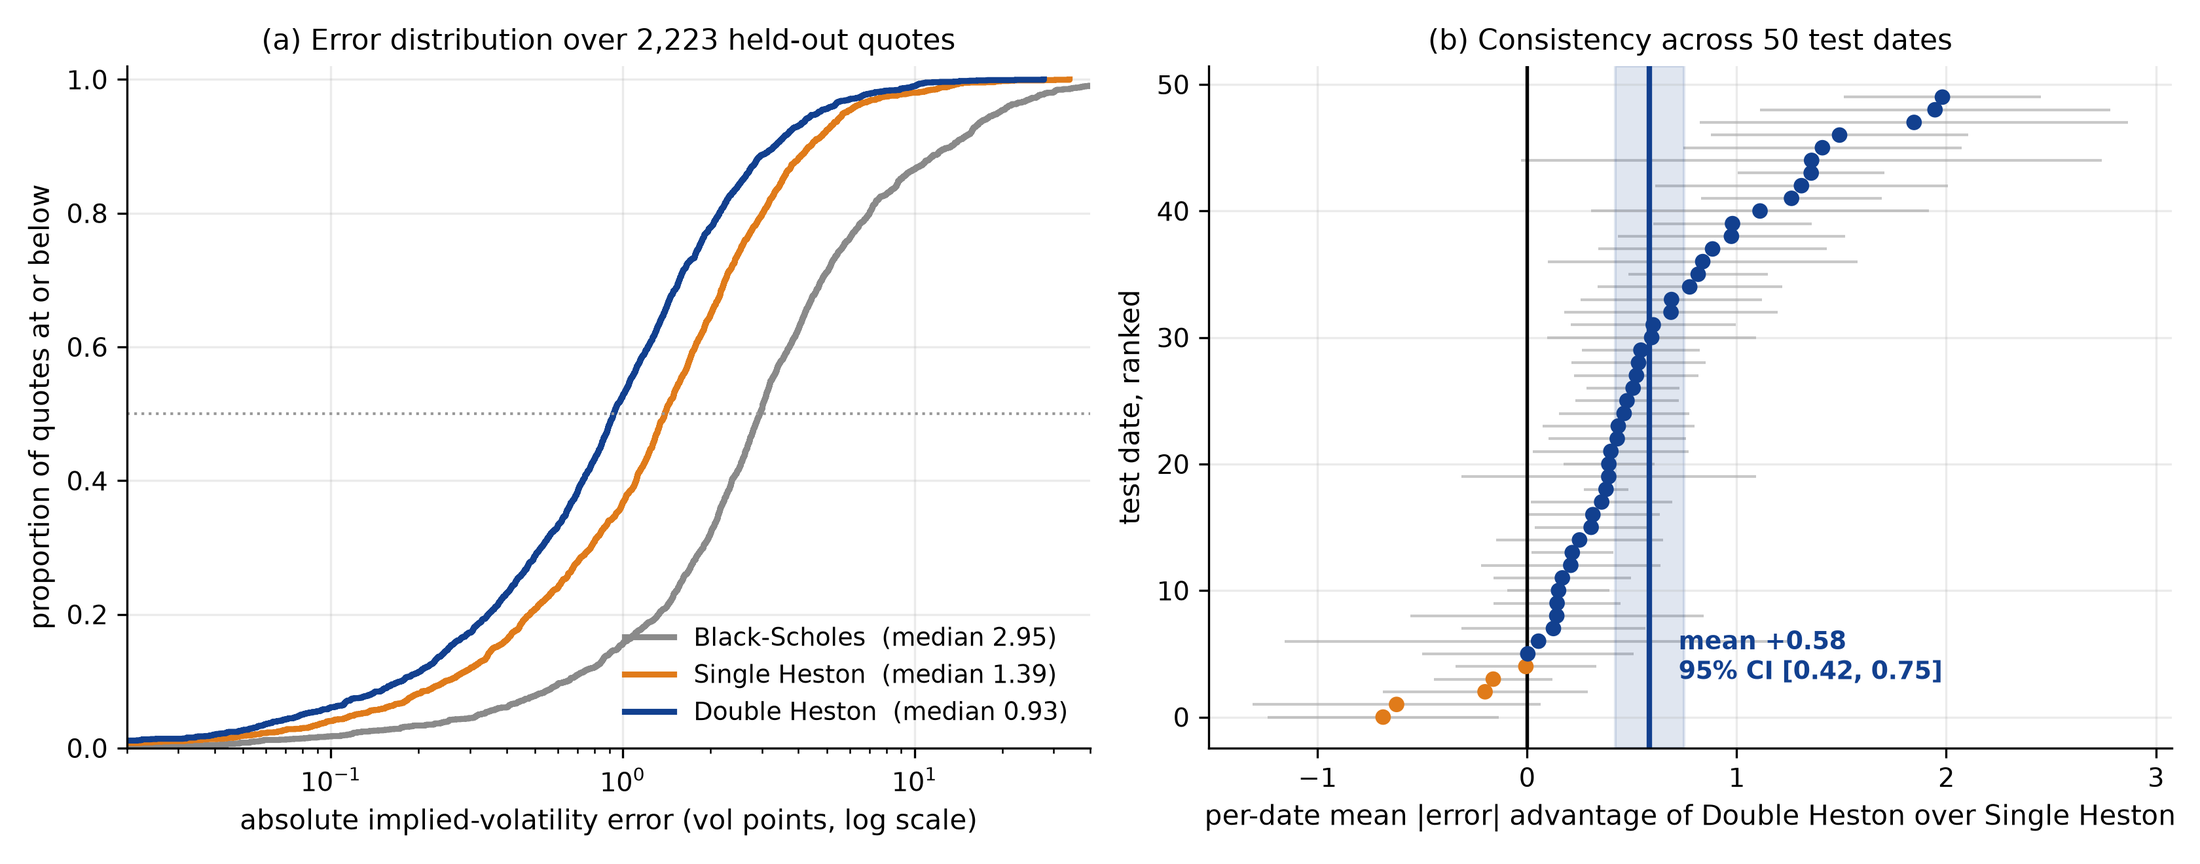
\includegraphics[width=\textwidth]{fig3_statistical_evidence.png}
\caption{Descriptive view of Bitcoin held-out errors, pooled over all 50 test
dates (2{,}223 quotes). (a)~Empirical cumulative distribution of absolute
implied-volatility error; Double Heston lies left of Single Heston at every
quantile. (b)~Per-date mean paired advantage of Double Heston over Single
Heston, ranked, with 95\% intervals; the shaded band is the cluster-bootstrap
interval for the overall mean. These are descriptive statistics pooled across
regimes and are not the pre-registered endpoint of Table~\ref{tab:results}.}
\label{fig:stats}
\end{figure}

\subsection{The Pattern Behind the Split}

The division is not random with respect to market structure.
Table~\ref{tab:markets} reports the median number of distinct expiries quoted
per evaluation date: Bitcoin quotes seven and Ether six, while Solana, XRP and
Hyperliquid quote about four. The two markets in which the second variance
factor pays are exactly the two that quote the most maturities.

This is what identifiability predicts. Two mean-reversion speeds can be
separated only if the data contain maturities at which their effects differ.
With four expiries, often with two or three clustered inside a month, a fast
and a slow factor produce nearly the same fitted surface, and the second factor
adds parameters without adding explanatory power. With six or seven expiries
spanning days to several months, the two time scales leave distinguishable
fingerprints and the extra factor earns its place.

\subsection{Illustration on a Single Surface}

Figure~\ref{fig:cvss} shows Bitcoin call prices against the underlying on a
representative date, with all three models calibrated to that date and
evaluated over the traded moneyness range. Prices are divided by the strike so
that quotes at different strikes are comparable. Single Heston lies above the
quotes and Black--Scholes below them, while Double Heston passes through them;
the Double-Heston price error is 4.7 times smaller than the better of the two
baselines. Figure~\ref{fig:cvstau} repeats the comparison against time to
maturity and shows the characteristic step in the Black--Scholes curve where it
switches between expiry knots, a structural consequence of granting it one
volatility per expiry. A single date is an illustration, not evidence; the
evidence is the pre-registered aggregate in Table~\ref{tab:results}.

\begin{figure}[htbp]
\centering
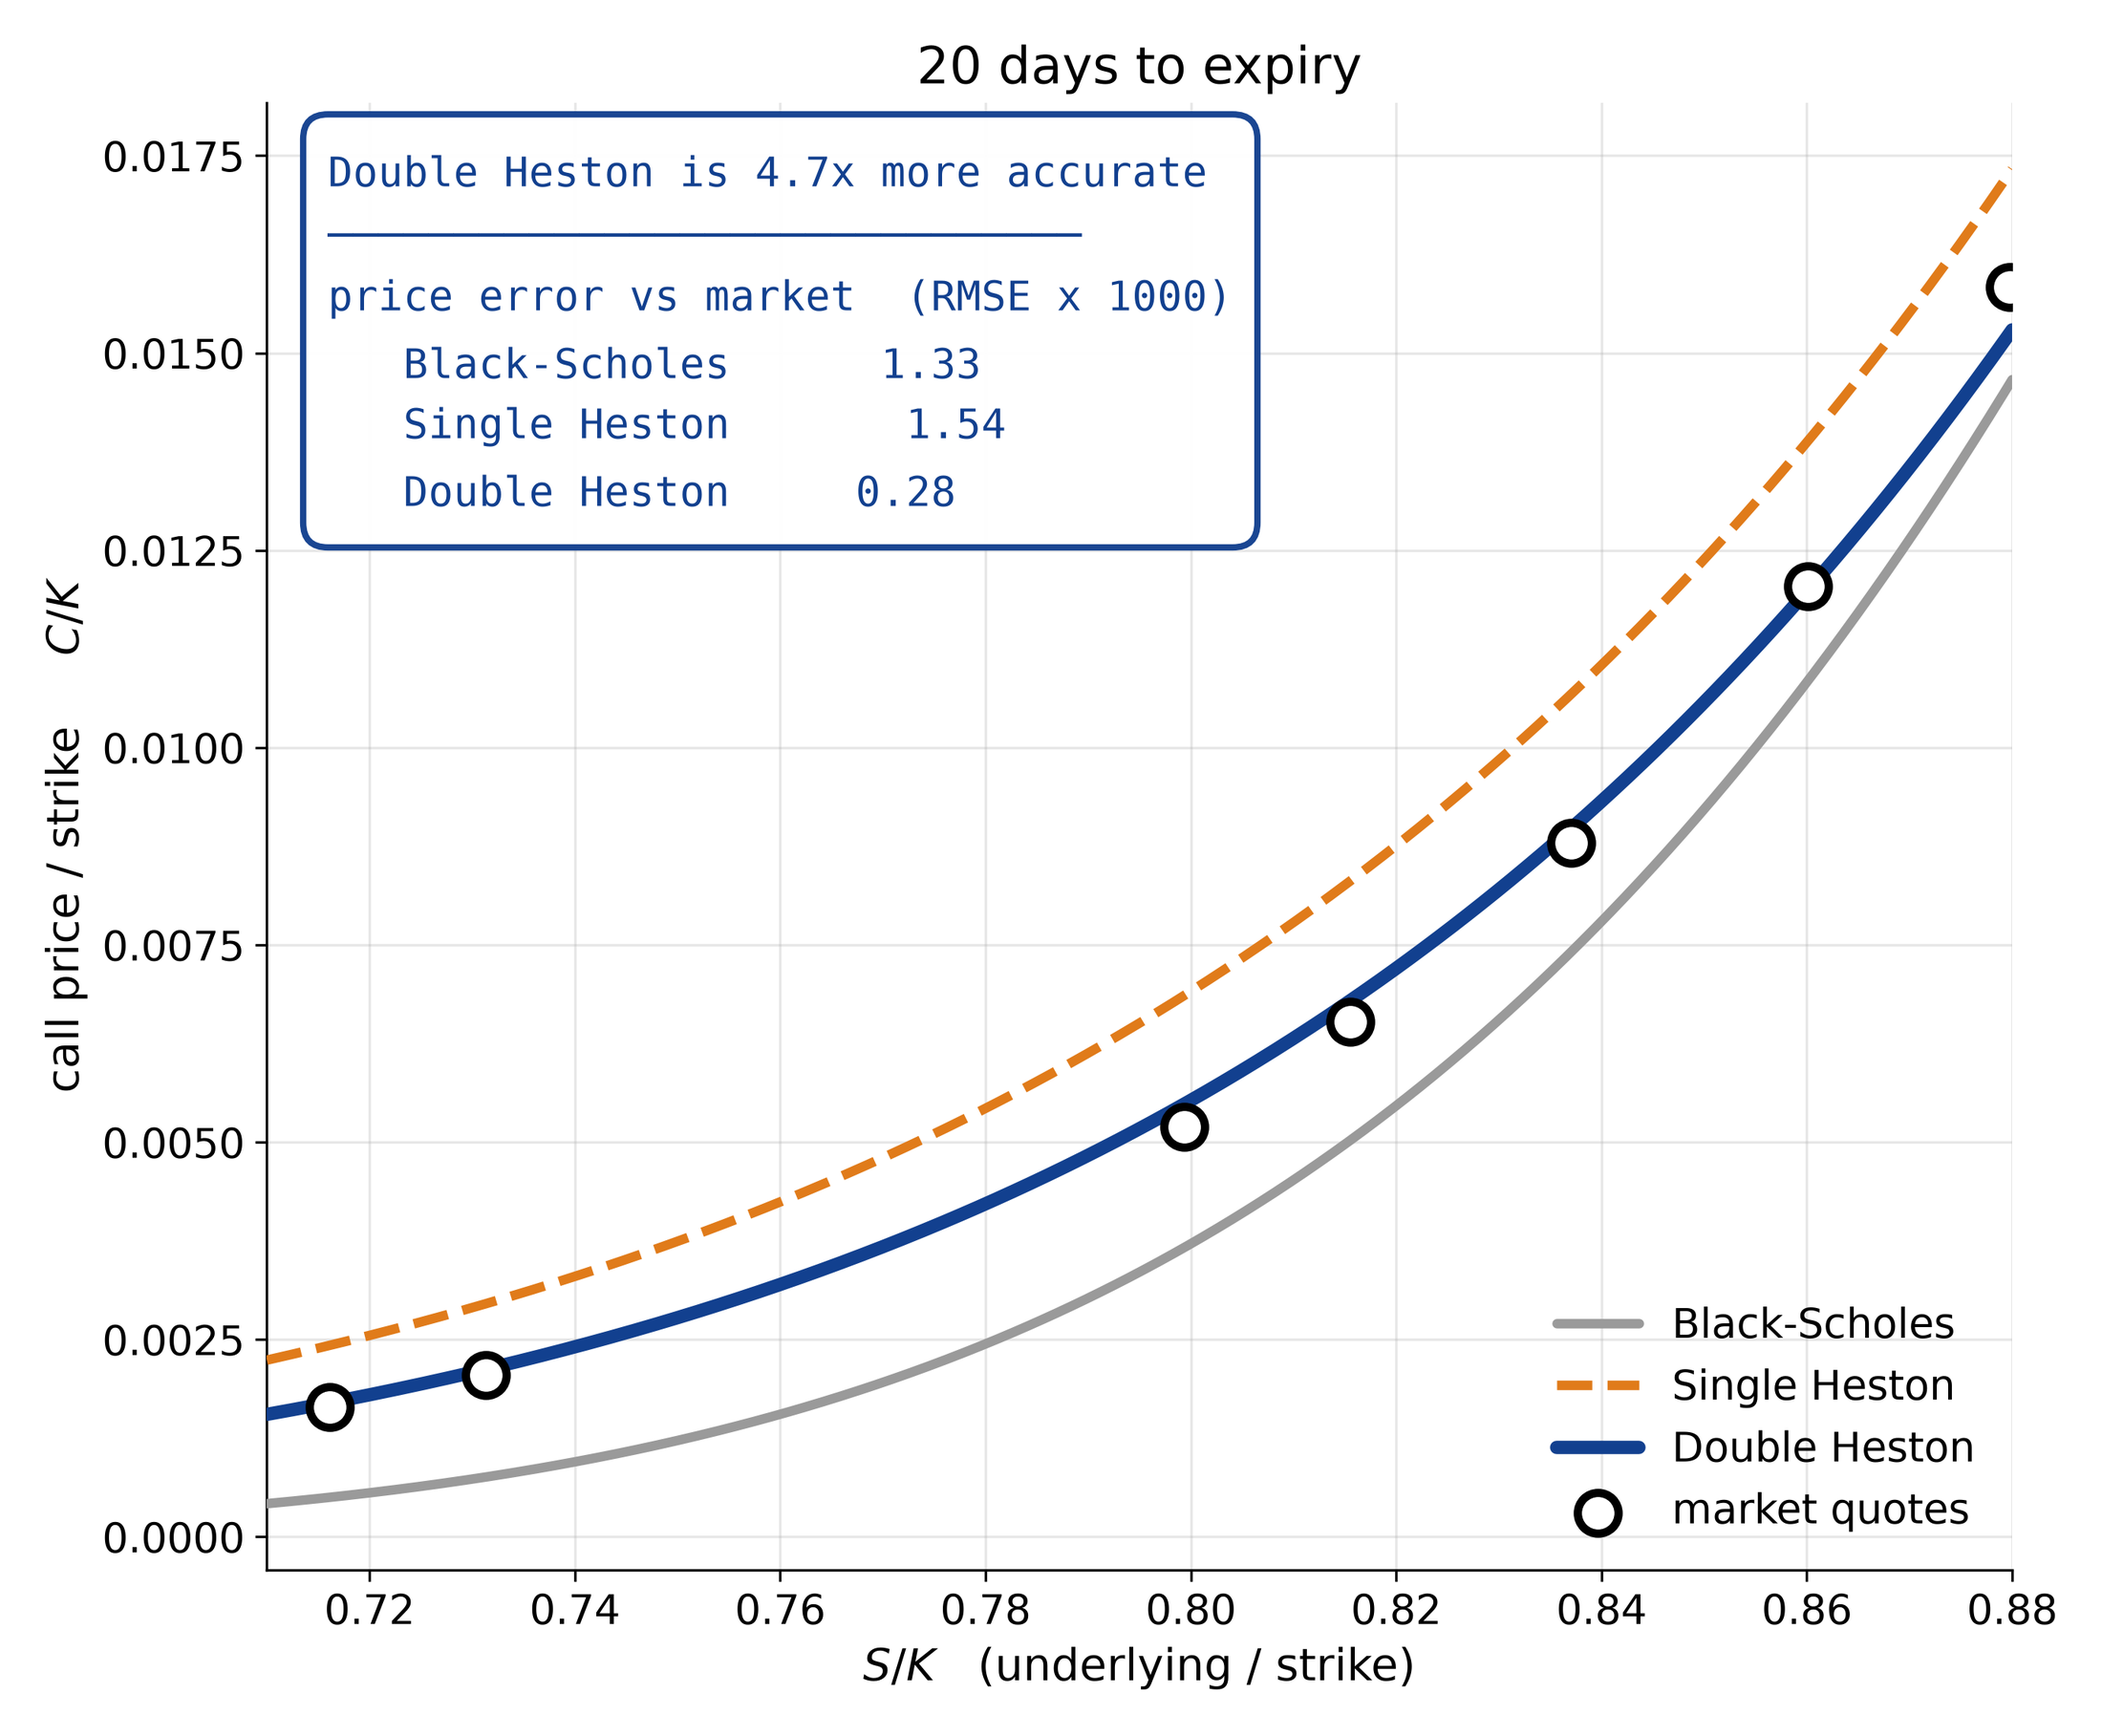
\includegraphics[width=0.78\textwidth]{fig1_C_vs_S.png}
\caption{Call price against underlying price for a held-out Bitcoin expiry,
with all three models calibrated to that date. Prices are divided by the strike
and the horizontal range is restricted to the region in which options carry
meaningful time value. Circles are market quotes.}
\label{fig:cvss}
\end{figure}

\begin{figure}[htbp]
\centering
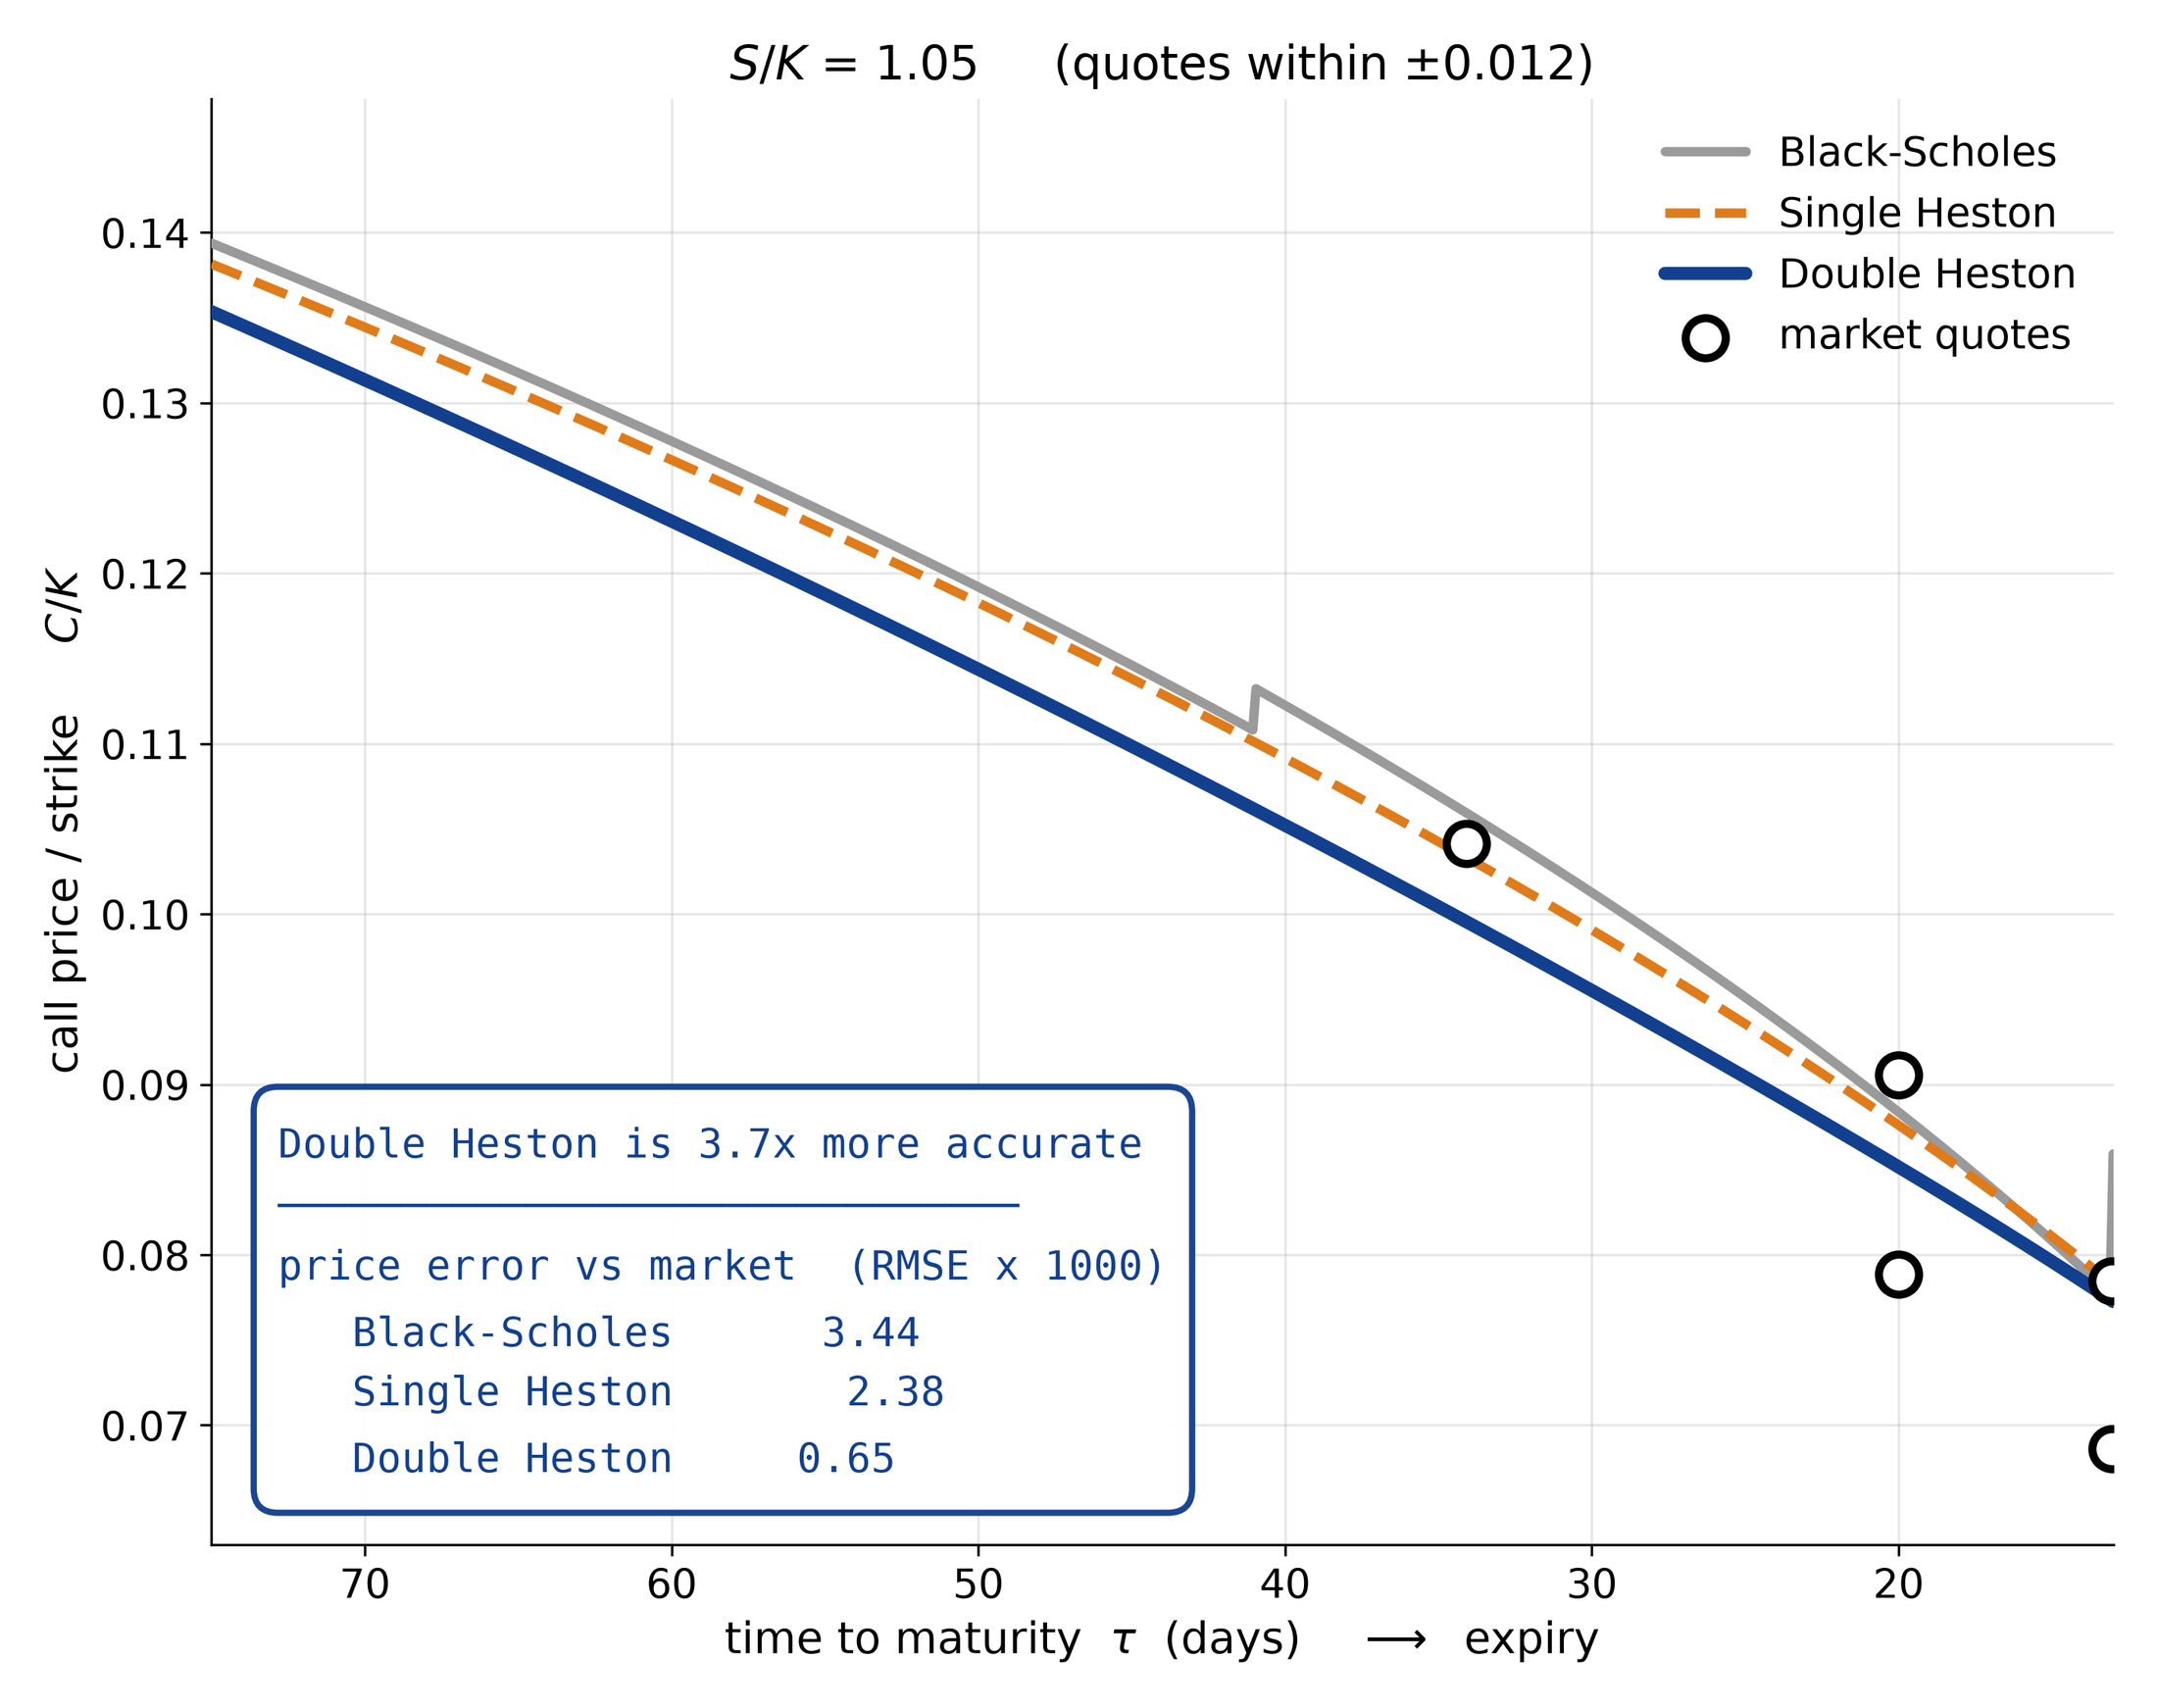
\includegraphics[width=0.78\textwidth]{fig2_C_vs_tau.png}
\caption{Call price against time to maturity at fixed moneyness on the same
date. Maturity decreases from left to right, so each curve decays towards its
payoff at expiry. The step in the Black--Scholes curve marks the point at which
it switches between expiry knots.}
\label{fig:cvstau}
\end{figure}

% =====================================================================
\FloatBarrier

Because a single surface can be chosen favourably, Figure~\ref{fig:range}
shows three surfaces side by side: the date on which Double Heston holds its
largest advantage, the date at the median advantage, and the date on which
Single Heston wins by the largest margin. On that last date the one-factor
model is the more accurate of the two. Reporting the unfavourable end of the
range is the reason the aggregate in Table~\ref{tab:results} should be read as
the result, and any single surface only as an illustration.

\begin{figure}[htbp]
\centering
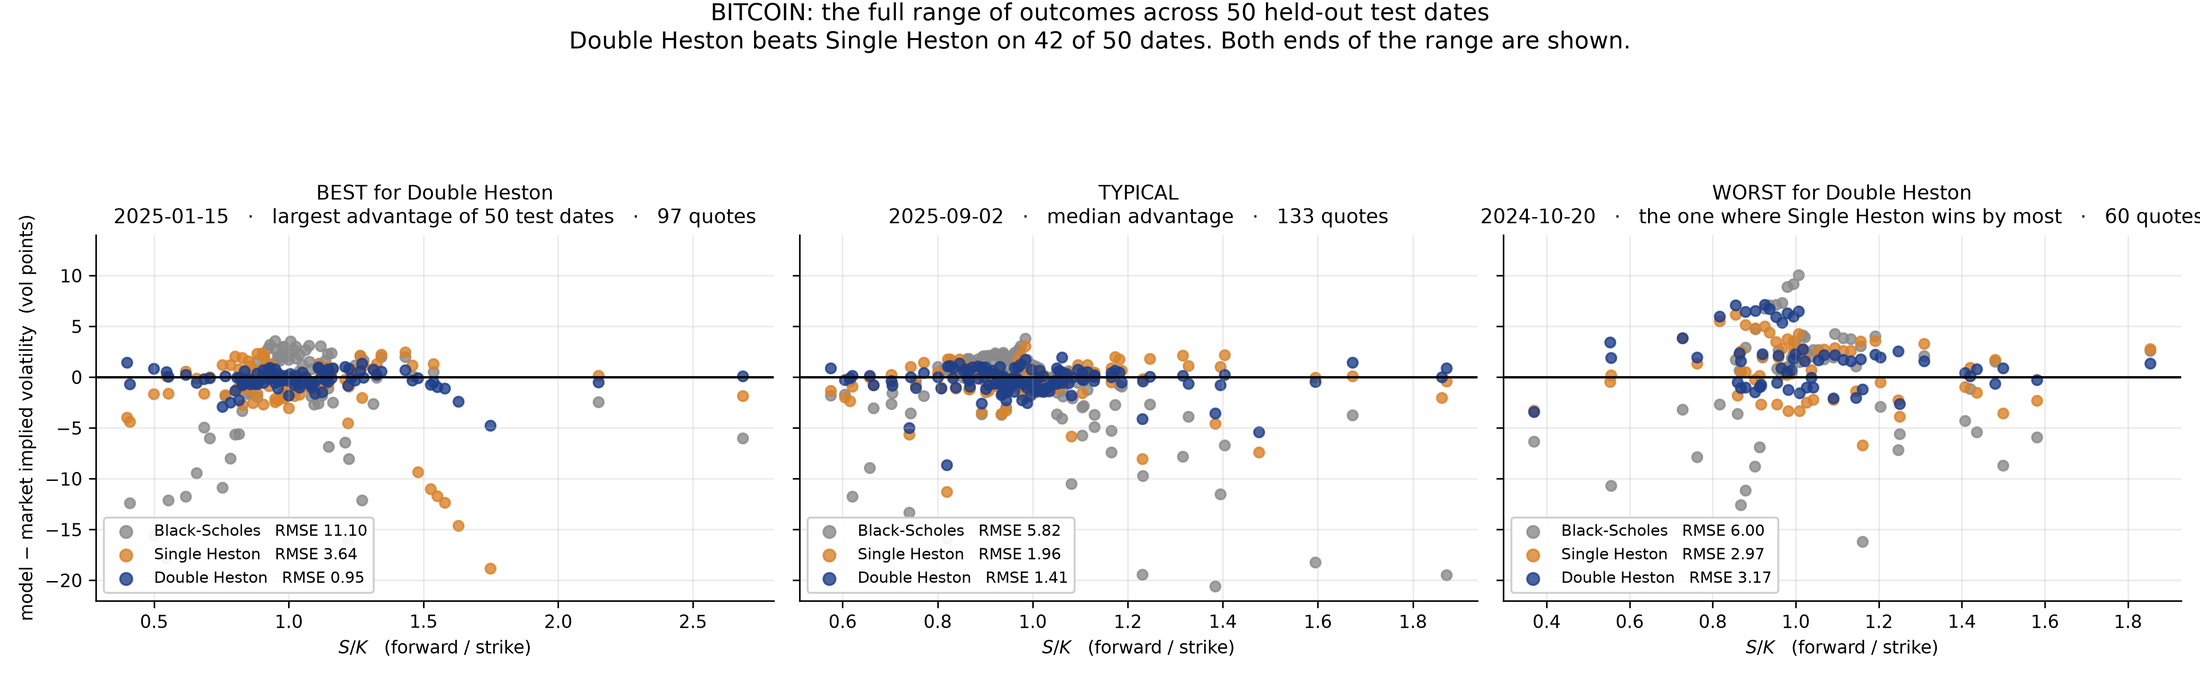
\includegraphics[width=\textwidth]{fig4_range_of_outcomes.png}
\caption{Range of single-date outcomes on Bitcoin, showing model minus market
implied volatility against moneyness. Left: the test date on which Double
Heston holds its largest advantage. Centre: the date at the median advantage.
Right: the date on which Single Heston wins by the largest margin. Both ends of
the range are shown so that the illustration in Figs.~\ref{fig:cvss}
and~\ref{fig:cvstau} is not mistaken for a typical case.}
\label{fig:range}
\end{figure}

\section{Discussion}

The headline result of most model-comparison papers is that the richer model
wins. Ours is that the richer model wins \emph{when the data can identify it},
and that this condition fails in three of the five markets examined.

This reframing matters for three reasons. First, it is actionable: a
practitioner deciding whether to move from one to two variance factors can
inspect the expiry count of the surface they actually trade, rather than rely
on a result obtained on a richer market. Second, it explains conflicting
results in the literature without attributing them to implementation
differences. Studies on major equity indices, where dozens of expiries are
listed, should find a two-factor advantage; studies on thin surfaces should
not. Both can be right. Third, it suggests the useful question is not ``which
model is better'' but ``how much structure can this surface support''. A model
that cannot be identified is not a better model whose benefits are hidden by
noise; it is an over-specified model whose extra parameters absorb noise.

The Solana calm-date result, where the one-factor model is significantly
better, is consistent with this reading. Over-specification does not merely
fail to help: it can actively hurt when the extra freedom fits features of the
calibration set that do not recur in the held-out set.

% =====================================================================
\section{Limitations}

The study covers cryptocurrency options on a single venue (Deribit). Crypto surfaces are
steeper and thinner than equity surfaces, so the specific threshold we observe,
roughly six expiries per day, should not be transferred to other asset classes
without re-testing. The mechanism---identifiability of two mean-reversion
speeds---should transfer; the numerical threshold need not.

Expiry count is not the only difference between these markets. Bitcoin and
Ether are also older, more liquid and have longer option histories. With five
markets we cannot fully separate maturity coverage from liquidity, and we do
not claim to. Expiry count is the variable that identifiability theory
singles out, and it orders the results without exception, but a larger
cross-section would be needed to isolate it.

Hyperliquid has the shortest history of the five markets: its 55 evaluation
dates fall inside one short listing window and are clustered by ISO week rather
than by volatility episode, so its 13 clusters are less independent than the
episode clusters used elsewhere. Our calibration
bounds bind in a large share of fits: the volatility-of-variance upper bound is
reached in 63 of 132 one-factor fits (48\%), and in 80 of 132 (61\%, slow
factor) and 76 of 132 (58\%, fast factor) two-factor fits. Relaxing those bounds after seeing the results is not
permitted under our own protocol, so we record it as the leading candidate
improvement for a future, independently pre-registered experiment. Finally, we
measure pricing accuracy on held-out quotes from the same day; forecasting,
hedging performance and economic value are separate questions.

% =====================================================================
\section{Conclusion}

We compared Black--Scholes, Heston and Double Heston on 16,186 held-out
option quotes from five cryptocurrency markets, under a design fixed and hashed before any
option data was seen. The two-factor model beat the constant-volatility
baseline everywhere, cutting median held-out implied-volatility error on
Bitcoin shock dates from 8.13 to 1.86 volatility points. Against the one-factor
model it won decisively on Bitcoin and Ether and failed to win on Solana, XRP
and Hyperliquid, with one market in which the simpler model was significantly
better.

The two markets in which the second variance factor paid are the two that quote
six to seven expiries per day; the three in which it did not quote about four.
We read this as an identifiability boundary rather than a property of the
model. The practical implication is that the choice between one and two
variance factors should be made by inspecting the surface, not only the model.
The methodological implication is that pre-registering the selection rule and
requiring two independent significance criteria changed our conclusions: two
results that a single test would have reported as wins did not survive both.

% =====================================================================
\begin{thebibliography}{99}

\bibitem{black1973}
Black, F., Scholes, M.: The pricing of options and corporate liabilities.
J. Polit. Econ. \textbf{81}(3), 637--654 (1973)

\bibitem{merton1973}
Merton, R.C.: Theory of rational option pricing. Bell J. Econ. Manag. Sci.
\textbf{4}(1), 141--183 (1973)

\bibitem{black1976}
Black, F.: The pricing of commodity contracts. J. Financ. Econ.
\textbf{3}(1--2), 167--179 (1976)

\bibitem{gatheral2006}
Gatheral, J.: The Volatility Surface: A Practitioner's Guide. Wiley, Hoboken
(2006)

\bibitem{heston1993}
Heston, S.L.: A closed-form solution for options with stochastic volatility
with applications to bond and currency options. Rev. Financ. Stud.
\textbf{6}(2), 327--343 (1993)

\bibitem{bakshi1997}
Bakshi, G., Cao, C., Chen, Z.: Empirical performance of alternative option
pricing models. J. Finance \textbf{52}(5), 2003--2049 (1997)

\bibitem{bates2000}
Bates, D.S.: Post-'87 crash fears in the S\&P 500 futures option market.
J. Econom. \textbf{94}(1--2), 181--238 (2000)

\bibitem{duffie2000}
Duffie, D., Pan, J., Singleton, K.: Transform analysis and asset pricing for
affine jump-diffusions. Econometrica \textbf{68}(6), 1343--1376 (2000)

\bibitem{chj2009}
Christoffersen, P., Heston, S., Jacobs, K.: The shape and term structure of the
index option smirk: why multifactor stochastic volatility models work so well.
Manag. Sci. \textbf{55}(12), 1914--1932 (2009)

\bibitem{carr1999}
Carr, P., Madan, D.B.: Option valuation using the fast Fourier transform.
J. Comput. Finance \textbf{2}(4), 61--73 (1999)

\bibitem{fang2008}
Fang, F., Oosterlee, C.W.: A novel pricing method for European options based on
Fourier-cosine series expansions. SIAM J. Sci. Comput. \textbf{31}(2),
826--848 (2008)

\bibitem{lord2010}
Lord, R., Kahl, C.: Complex logarithms in Heston-like models. Math. Finance
\textbf{20}(4), 671--694 (2010)

\bibitem{cui2017}
Cui, Y., del Ba\~{n}o Rollin, S., Germano, G.: Full and fast calibration of the
Heston stochastic volatility model. Eur. J. Oper. Res. \textbf{263}(2),
625--638 (2017)

\bibitem{feller1951}
Feller, W.: Two singular diffusion problems. Ann. Math. \textbf{54}(1),
173--182 (1951)

\bibitem{madan2019}
Madan, D.B., Reyners, S., Schoutens, W.: Advanced model calibration on bitcoin
options. Digit. Finance \textbf{1}, 117--137 (2019)

\bibitem{hou2020}
Hou, A.J., Wang, W., Chen, C.Y.H., H\"{a}rdle, W.K.: Pricing cryptocurrency
options. J. Financ. Econom. \textbf{18}(2), 250--279 (2020)

\bibitem{alexander2021}
Alexander, C., Imeraj, A.: The Bitcoin VIX and its variance risk premium.
J. Altern. Invest. \textbf{23}(4), 84--109 (2021)

\bibitem{alexander2023}
Alexander, C., Imeraj, A.: Delta hedging bitcoin options with a smile.
Quant. Finance \textbf{23}(5), 799--817 (2023)

\bibitem{wilcoxon1945}
Wilcoxon, F.: Individual comparisons by ranking methods. Biom. Bull.
\textbf{1}(6), 80--83 (1945)

\bibitem{efron1979}
Efron, B.: Bootstrap methods: another look at the jackknife. Ann. Stat.
\textbf{7}(1), 1--26 (1979)

\bibitem{cameron2008}
Cameron, A.C., Gelbach, J.B., Miller, D.L.: Bootstrap-based improvements for
inference with clustered errors. Rev. Econ. Stat. \textbf{90}(3), 414--427
(2008)

\bibitem{nosek2018}
Nosek, B.A., Ebersole, C.R., DeHaven, A.C., Mellor, D.T.: The preregistration
revolution. Proc. Natl. Acad. Sci. \textbf{115}(11), 2600--2606 (2018)

\end{thebibliography}

\end{document}
